% LaTeX2e Template by Stephen Iota (https://stepheniota.github.io/)
% last updated: Aug. 2018

% for papers
%\documentclass[aps,onecolumn,superscriptaddress]{revtex4-1}

% https://www-d0.fnal.gov/Run2Physics/WWW/templates/revtex4.pdf
% https://cdn.journals.aps.org/files/revtex/auguide4-1.pdf
% for revTeX4-1 class options

% for other
\documentclass{article}
\usepackage[margin=1in]{geometry}

%%%%%%%%%%%%%%%%
%%% Packages %%%
%%%%%%%%%%%%%%%%

\usepackage[utf8]{inputenc}
%\usepackage{amsmath}
%\usepackage{amssymb}
%\usepackage{amsfonts}
\usepackage{graphicx}
\usepackage{enumitem}
\graphicspath{{figures/}} % set directory for figures
\usepackage[dvipsnames]{xcolor} % for colored links


% always put this at the end
\usepackage[
	colorlinks=true,
	citecolor=green!50!black,
	linkcolor=NavyBlue!75!black,
	urlcolor=green!50!black,
	hypertexnames=false]{hyperref} 

 
 %%%%%%%%%%%%%%%%%%
 %% New Commands %%
 %%%%%%%%%%%%%%%%%%
 
\newcommand{\email}[1]{\texttt{\href{mailto:#1}{#1}}}
 
%----------------------------------------------------
%%%%%%%%%%%%%%%%%%
%% Front Matter %%
%%%%%%%%%%%%%%%%%%

% no page numbers
%\pagenumbering{gobble}


%%%%%%%%%%%%%
%%% Title %%%
%%%%%%%%%%%%%
\begin{document}

\begin{center}

\Large{\textsc{Worksheet 1}: \textbf{Charges and the $\vec{E}$ Field}}

\end{center}

\vspace{.5mm}

%%%%%%%%%%
%% INFO %%
%%%%%%%%%%

\begin{tabular}{rl}

\textsc{Course}:
&
Physics 40C (Fall 2018), Dr.~Laura Sales
\\
\textsc{SI Leader}
&
Stephen Iota (\email{siota001@ucr.edu})
\\
\textsc{Date}:
&
October 4, 2018
\end{tabular}

%%%%%%%%%%%%%%
%% PROBLEMS %%
%%%%%%%%%%%%%%


\section{Conductors \& Insulators}

\begin{enumerate}[label=(\alph*)]

	\item What makes an insulator different from a conductor?
	\item Can an insulator still become electrically charged? Discuss an experiment you could do to determine the answer. 
	\item Two neutral metal spheres on wood stands are touching. A negatively charged rod is held directly above the top of the left sphere, not quite touching it. While the rod is there, the right sphere is moved so that the spheres no longer touch. Then the rod is withdrawn. Afterward, what is the charge state of each sphere? Use charge diagrams to explain your answer.
	
\end{enumerate}


\section{Understanding $\vec{E}$}

\begin{enumerate}[label=(\alph*)]

\item Describe, in as much detail possible, what the electric field ($\vec{E}$) is.
\begin{itemize}
	\item What are the units of the $\vec{E}$ field?
	\item What is the equation that governs the $\vec{E}$ field? Units?
	\item What are some other examples of fields in physics? Similarities/differences? 
\end{itemize}
 

\item An electron is placed at the position marked by the dot. What direction is the force on the electron?



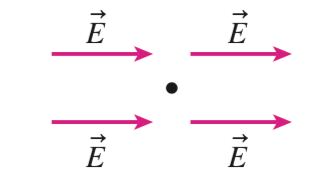
\includegraphics[width=.3\linewidth]{W1_Fig1}


\item An electron experiences a force of magnitude $F$ when it is $x$ distance away from a very long, charged wire with a linear charge density $\lambda$. If the charge density is doubled, at what distance from the wire will a proton experience a force of the same magnitude $F$? 

\item Two protons are $2.0$ fm apart.
\begin{itemize}
	\item What is the magnitude of the electric force on one proton due to the other proton?
	\item What is the magnitude of the gravitational force on one proton due to the other proton?
\end{itemize} 


\item Write the electric field at point $P$ in component form.

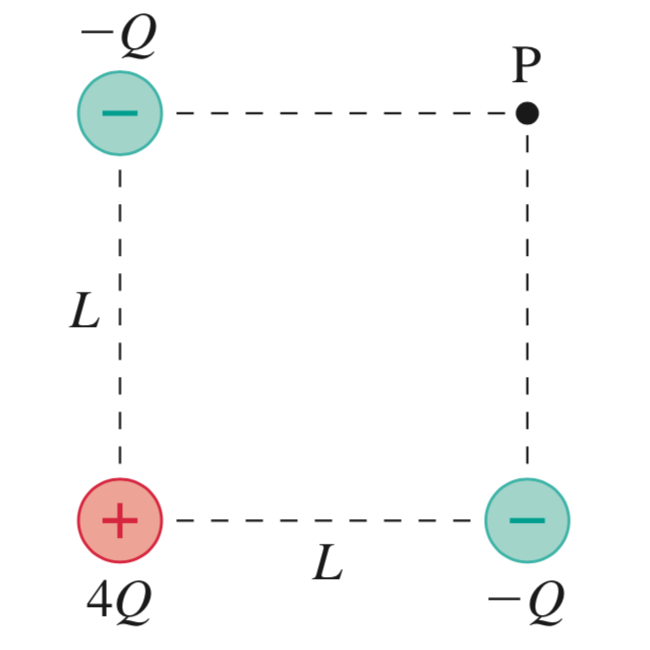
\includegraphics[width=.3\linewidth]{W1_Fig2}

\end{enumerate}

\section{The Electric Dipole $\vec{p}$} 

\begin{enumerate}[label=(\alph*)]
	\item Write down the equations for $\vec{E}_{dipole}$ from the textbook.
	
	\item What happens to an electric dipole in a {\bfseries uniform} electric field?
	
\end{enumerate}


\section{Charged Particle Field Interaction}

An electron is at the origin at $t = 0$ with an initial velocity $\vec{v} = 2\vec{x} + 1\vec{y}$ m/s, moving through a uniform electric field $\vec{E} = 3\vec{y}$ N/C. What is the electron's position at $t = 5$ s?
\\

\noindent 
Hint: Do you remember kinematics from 40A?



\end{document}